\documentclass[11pt,fleqn, openany]{book} % Default font size and left-justified equations

%%%%%%%%%%%%%%%%%%%%%%%%%%%%%%%%%%%%%%%%%
% The Legrand Orange Book
% Structural Definitions File
% Version 2.1 (26/09/2018)
%
% Original author:
% Mathias Legrand (legrand.mathias@gmail.com) with modifications by:
% Vel (vel@latextemplates.com)
% 
% This file was downloaded from:
% http://www.LaTeXTemplates.com
%
% License:
% CC BY-NC-SA 3.0 (http://creativecommons.org/licenses/by-nc-sa/3.0/)
%
%%%%%%%%%%%%%%%%%%%%%%%%%%%%%%%%%%%%%%%%%

%----------------------------------------------------------------------------------------
%	VARIOUS REQUIRED PACKAGES AND CONFIGURATIONS
%----------------------------------------------------------------------------------------

\usepackage[table]{xcolor}

\usepackage{graphicx}
\usepackage{tabularx} % Required for including pictures
\usepackage{pgf,tikz,tkz-tab,eurosym,yhmath, stmaryrd}
\usepackage{pgfplots}
\usepackage{mathrsfs}
\usetikzlibrary{patterns}
\usetikzlibrary{trees}
\graphicspath{{../../Pictures/}}
\usepackage{multicol} 


\usepackage[english]{babel} % English language/hyphenation
\usepackage{icomma}
\usepackage{enumitem} % Customize lists
\setlist{nolistsep, nosep, nolistsep} % Reduce spacing between bullet points and numbered lists

\usepackage{booktabs} % Required for nicer horizontal rules in tables

 % Required for specifying colors by name


\definecolor{ocre}{RGB}{243,102,25} % Define the orange color used for highlighting throughout the book

\usepackage{listings}

\definecolor{codegreen}{rgb}{0,0.6,0}
\definecolor{codegray}{rgb}{0.5,0.5,0.5}
\definecolor{codepurple}{rgb}{0.58,0,0.82}
\definecolor{backcolour}{rgb}{0.95,0.95,0.92}

\lstdefinestyle{mystyle}{
    backgroundcolor=\color{backcolour},   
    commentstyle=\color{codegreen},
    keywordstyle=\color{magenta},
    numberstyle=\tiny\color{codegray},
    stringstyle=\color{codepurple},
    basicstyle=\ttfamily\footnotesize,
    breakatwhitespace=false,         
    breaklines=true,                 
    captionpos=b,                    
    keepspaces=true,                 
    numbers=left,                    
    numbersep=5pt,                  
    showspaces=false,                
    showstringspaces=false,
    showtabs=false,                  
    tabsize=2
}

\lstset{style=mystyle}

%----------------------------------------------------------------------------------------
% Paramétrage XSIM
%----------------------------------------------------------------------------------------

\usepackage[no-files]{xsim}


\DeclareExerciseEnvironmentTemplate{myex}{%
    \textbf{%
      \hypertarget{ex:\ExerciseID}{\sffamily{\ensuremath{\blacktriangleright}} Exercice \GetExerciseProperty{counter} \GetExerciseProperty{subtitle} --}
      \hyperlink{sol:\ExerciseID}{Voir le corrigé}%
    }\par
}{\par\smallskip}

\DeclareExerciseEnvironmentTemplate{mysol}{%
    \textbf{%
      \hypertarget{sol:\ExerciseID}{\sffamily{\ensuremath{\blacktriangleright}} Correction \GetExerciseProperty{counter} --}
      \hyperlink{ex:\ExerciseID}{Voir l'énoncé}%
    }\par
}{\par\medskip}

\xsimsetup{
  exercise/template = myex ,
  solution/template = mysol 
}

%Collection exercices

\DeclareExerciseTagging{topic}

\xsimsetup{collect}

%----------------------------------------------------------------------------------------
% SYMBOLES
%----------------------------------------------------------------------------------------

\newcommand\imCMsym[4][\mathord]{%
  \DeclareFontFamily{U} {#2}{}
  \DeclareFontShape{U}{#2}{m}{n}{
    <-6> #25
    <6-7> #26
    <7-8> #27
    <8-9> #28
    <9-10> #29
    <10-12> #210
    <12-> #212}{}
  \DeclareSymbolFont{CM#2} {U} {#2}{m}{n}
  \DeclareMathSymbol{#4}{#1}{CM#2}{#3}
}
\newcommand\alsoimCMsym[4][\mathord]{\DeclareMathSymbol{#4}{#1}{CM#2}{#3}}

\imCMsym{cmmi}{124}{\CMjmath}

\newcommand{\Oij}{(O\,;\,\vec{\imath}\,,\, \vec{\CMjmath} )}
\newcommand{\Oijk}{(O\,;\,\vec{\imath}\,,\, \vec{\CMjmath}\,,\,\vec{k})}

\newcommand\e{\mathrm{e}}
\newcommand\R{\mathbb{R}}
\newcommand\N{\mathbb{N}}


%----------------------------------------------------------------------------------------
%	MARGINS
%----------------------------------------------------------------------------------------

\usepackage{geometry} % Required for adjusting page dimensions and margins

\geometry{
	paper=a4paper, % Paper size, change to letterpaper for US letter size
	top=3cm, % Top margin
	bottom=3cm, % Bottom margin
	left=2cm, % Left margin
	right=2cm, % Right margin
	headheight=14pt, % Header height
	footskip=1.4cm, % Space from the bottom margin to the baseline of the footer
	headsep=10pt, % Space from the top margin to the baseline of the header
	%showframe, % Uncomment to show how the type block is set on the page
}

\setlength{\parindent}{0pt}
\parskip=5pt



%----------------------------------------------------------------------------------------
%	FONTS
%----------------------------------------------------------------------------------------

\usepackage{avant} % Use the Avantgarde font for headings
\usepackage{times} % Use the Times font for headings
\usepackage{mathptmx} % Use the Adobe Times Roman as the default text font together with math symbols from the Sym­bol, Chancery and Com­puter Modern fonts

%\usepackage{microtype} % Slightly tweak font spacing for aesthetics
%\usepackage[utf8]{inputenc} % Required for including letters with accents
\usepackage[T1]{fontenc} % Use 8-bit encoding that has 256 glyphs

%----------------------------------------------------------------------------------------
%	BIBLIOGRAPHY AND INDEX
%----------------------------------------------------------------------------------------

\usepackage[style=numeric,citestyle=numeric,sorting=nyt,sortcites=true,autopunct=true,babel=hyphen,hyperref=true,abbreviate=false,backref=true,backend=biber]{biblatex}
\addbibresource{bibliography.bib} % BibTeX bibliography file
\defbibheading{bibempty}{}

\usepackage{calc} % For simpler calculation - used for spacing the index letter headings correctly
\usepackage{makeidx} % Required to make an index
\makeindex % Tells LaTeX to create the files required for indexing

%----------------------------------------------------------------------------------------
%	MAIN TABLE OF CONTENTS
%----------------------------------------------------------------------------------------

\usepackage{titletoc} % Required for manipulating the table of contents

\contentsmargin{0cm} % Removes the default margin

% Part text styling (this is mostly taken care of in the PART HEADINGS section of this file)
\titlecontents{part}
	[0cm] % Left indentation
	{\addvspace{20pt}\bfseries} % Spacing and font options for parts
	{}
	{}
	{}

% Chapter text styling
\titlecontents{chapter}
	[1.25cm] % Left indentation
	{\addvspace{12pt}\large\sffamily\bfseries} % Spacing and font options for chapters
	{\color{ocre!60}\contentslabel[\Large\thecontentslabel]{1.25cm}\color{ocre}} % Formatting of numbered sections of this type
	{\color{ocre}} % Formatting of numberless sections of this type
	{\color{ocre!60}\normalsize\;\titlerule*[.5pc]{.}\;\thecontentspage} % Formatting of the filler to the right of the heading and the page number

% Section text styling
\titlecontents{section}
	[1.25cm] % Left indentation
	{\addvspace{3pt}\sffamily\bfseries} % Spacing and font options for sections
	{\contentslabel[\thecontentslabel]{1.25cm}} % Formatting of numbered sections of this type
	{} % Formatting of numberless sections of this type
	{\hfill\color{black}\thecontentspage} % Formatting of the filler to the right of the heading and the page number

% Subsection text styling
\titlecontents{subsection}
	[1.25cm] % Left indentation
	{\addvspace{1pt}\sffamily\small} % Spacing and font options for subsections
	{\contentslabel[\thecontentslabel]{1.25cm}} % Formatting of numbered sections of this type
	{} % Formatting of numberless sections of this type
	{\ \titlerule*[.5pc]{.}\;\thecontentspage} % Formatting of the filler to the right of the heading and the page number

% Figure text styling
\titlecontents{figure}
	[1.25cm] % Left indentation
	{\addvspace{1pt}\sffamily\small} % Spacing and font options for figures
	{\thecontentslabel\hspace*{1em}} % Formatting of numbered sections of this type
	{} % Formatting of numberless sections of this type
	{\ \titlerule*[.5pc]{.}\;\thecontentspage} % Formatting of the filler to the right of the heading and the page number

% Table text styling
\titlecontents{table}
	[1.25cm] % Left indentation
	{\addvspace{1pt}\sffamily\small} % Spacing and font options for tables
	{\thecontentslabel\hspace*{1em}} % Formatting of numbered sections of this type
	{} % Formatting of numberless sections of this type
	{\ \titlerule*[.5pc]{.}\;\thecontentspage} % Formatting of the filler to the right of the heading and the page number

%----------------------------------------------------------------------------------------
%	MINI TABLE OF CONTENTS IN PART HEADS
%----------------------------------------------------------------------------------------

% Chapter text styling
\titlecontents{lchapter}
	[0em] % Left indentation
	{\addvspace{15pt}\large\sffamily\bfseries} % Spacing and font options for chapters
	{\color{ocre}\contentslabel[\Large\thecontentslabel]{1.25cm}\color{ocre}} % Chapter number
	{}  
	{\color{ocre}\normalsize\sffamily\bfseries\;\titlerule*[.5pc]{.}\;\thecontentspage} % Page number

% Section text styling
\titlecontents{lsection}
	[0em] % Left indentation
	{\sffamily\small} % Spacing and font options for sections
	{\contentslabel[\thecontentslabel]{1.25cm}} % Section number
	{}
	{}

% Subsection text styling (note these aren't shown by default, display them by searchings this file for tocdepth and reading the commented text)
\titlecontents{lsubsection}
	[.5em] % Left indentation
	{\sffamily\footnotesize} % Spacing and font options for subsections
	{\contentslabel[\thecontentslabel]{1.25cm}}
	{}
	{}

%----------------------------------------------------------------------------------------
%	HEADERS AND FOOTERS
%----------------------------------------------------------------------------------------


\usepackage{fancyhdr} % Required for header and footer configuration

\pagestyle{fancy}
\renewcommand{\chaptermark}[1]{\markboth{\sffamily\normalsize\bfseries\ \thechapter.\ #1}{}} % Chapter text font settings
\renewcommand{\sectionmark}[1]{\markright{\sffamily\normalsize\thesection\hspace{5pt}#1}{}} % Section text font settings
\fancyhf{} \fancyhead[LE,RO]{\sffamily\normalsize\thepage} % Font setting for the page number in the header
\fancyhead[LO]{\rightmark} % Print the nearest section name on the left side of odd pages
\fancyhead[RE]{\leftmark} % Print the current chapter name on the right side of even pages

\fancyfoot[L]{Jason LAPEYRONNIE}
\fancyfoot[R]{\href{http://mathoutils.fr}{http://mathoutils.fr}} % Uncomment to include a footer

\renewcommand{\headrulewidth}{0.5pt} % Thickness of the rule under the header
\renewcommand{\footrulewidth}{0.5pt} % Thickness of the rule under the header

\fancypagestyle{plain}{% Style for when a plain pagestyle is specified
	\fancyhead{}\renewcommand{\headrulewidth}{0pt}%
}

% Removes the header from odd empty pages at the end of chapters
\makeatletter
\renewcommand{\cleardoublepage}{
\clearpage\ifodd\c@page\else
\hbox{}
\vspace*{\fill}
\thispagestyle{empty}
\newpage
\fi}

%----------------------------------------------------------------------------------------
%	THEOREM STYLES
%----------------------------------------------------------------------------------------

\usepackage{amsmath,amsfonts,amssymb,amsthm} % For math equations, theorems, symbols, etc

\newcommand{\intoo}[2]{\mathopen{]}#1\,;#2\mathclose{[}}
\newcommand{\ud}{\mathop{\mathrm{{}d}}\mathopen{}}
\newcommand{\intff}[2]{\mathopen{[}#1\,;#2\mathclose{]}}
\renewcommand{\qedsymbol}{$\blacksquare$}
\newtheorem{notation}{Notation}[section]

% Boxed/framed environments
\newtheoremstyle{ocrenumbox}% Theorem style name
{0pt}% Space above
{0pt}% Space below
{\normalfont}% Body font
{}% Indent amount
{\small\bf\sffamily\color{ocre}}% Theorem head font
{\;:\;}% Punctuation after theorem head
{0.25em}% Space after theorem head
{\small\sffamily\color{ocre}\thmname{#1}\nobreakspace\thmnumber{\@ifnotempty{#1}{}\@upn{#2}}% Theorem text (e.g. Theorem 2.1)
\thmnote{\nobreakspace\the\thm@notefont\sffamily\bfseries\color{black}---\nobreakspace#3}} % Optional theorem note

\newtheoremstyle{blacknumex}% Theorem style name
{5pt}% Space above
{10pt}% Space below
{\normalfont}% Body font
{} % Indent amount
{\small\bf\sffamily}% Theorem head font
{\;:\;}% Punctuation after theorem head
{0.25em}% Space after theorem head
{\small\sffamily{\tiny\ensuremath{\blacksquare}}\nobreakspace\thmname{#1}\nobreakspace\thmnumber{\@ifnotempty{#1}{}\@upn{#2}}% Theorem text (e.g. Theorem 2.1)
\thmnote{\nobreakspace\the\thm@notefont\sffamily\bfseries---\nobreakspace#3}}% Optional theorem note

\newtheoremstyle{blacknumexo}% Theorem style name
{15pt}% Space above
{10pt}% Space below
{\normalfont}% Body font
{} % Indent amount
{\small\bf\sffamily}% Theorem head font
{}% Punctuation after theorem head
{0.5em}% Space after theorem head
{\small\sffamily{\ensuremath{\blacktriangleright}}\nobreakspace\thmname{#1}\nobreakspace\thmnumber{\@ifnotempty{#1}{}\@upn{#2}}% Theorem text (e.g. Theorem 2.1)
\thmnote{\nobreakspace\the\thm@notefont\sffamily\bfseries---\nobreakspace#3} \\}% Optional theorem note



\newtheoremstyle{blacknumbox} % Theorem style name
{0pt}% Space above
{5pt}% Space below
{}% Body font
{}% Indent amount
{\large\bf\sffamily}% Theorem head font
{\;:\;}% Punctuation after theorem head
{0.25em}% Space after theorem head
{\small\sffamily\thmname{#1}\nobreakspace\thmnumber{\@ifnotempty{#1}{}\@upn{#2}}% Theorem text (e.g. Theorem 2.1)
\thmnote{\nobreakspace\the\thm@notefont\sffamily\bfseries---\nobreakspace#3}}% Optional theorem note

% Non-boxed/non-framed environments
\newtheoremstyle{ocrenum}% Theorem style name
{5pt}% Space above
{5pt}% Space below
{\normalfont}% Body font
{}% Indent amount
{\small\bf\sffamily\color{ocre}}% Theorem head font
{\;:\;}% Punctuation after theorem head
{0.25em}% Space after theorem head
{\small\sffamily\color{ocre}\thmname{#1}\nobreakspace\thmnumber{\@ifnotempty{#1}{}\@upn{#2}}% Theorem text (e.g. Theorem 2.1)
\thmnote{\nobreakspace\the\thm@notefont\sffamily\bfseries\color{black}---\nobreakspace#3}} % Optional theorem note
\makeatother

% Defines the theorem text style for each type of theorem to one of the three styles above
\newcounter{dummy} 
\newcounter{thm}
\newcounter{correction}
\newcounter{qst}
\theoremstyle{ocrenumbox}
\newtheorem{theoremeT}[dummy]{Théorème}
\newtheorem{exerciseT}{Propriété}
\newtheorem{principeT}{Principe}
\theoremstyle{blacknumex}
\newtheorem{exampleT}{Exemple}
\theoremstyle{blacknumexo}
\newtheorem{exo}[thm]{Exercice}
\newtheorem{corr}[correction]{Correction}
\newtheorem{quest}[qst]{Question}
\theoremstyle{blacknumbox}
\newtheorem{vocabulary}{Vocabulary}[section]
\newtheorem{definitionT}{Définition}
\newtheorem{corollaryT}[dummy]{Corollary}
\theoremstyle{ocrenum}
\newtheorem{proofT}[dummy]{Démonstration}


%----------------------------------------------------------------------------------------
%	DEFINITION OF COLORED BOXES
%----------------------------------------------------------------------------------------

\RequirePackage[framemethod=default]{mdframed} % Required for creating the theorem, definition, exercise and corollary boxes

% Theorem box
\newmdenv[skipabove=7pt,
skipbelow=7pt,
backgroundcolor=black!5,
linecolor=ocre,
innerleftmargin=5pt,
innerrightmargin=5pt,
innertopmargin=10pt,
leftmargin=0cm,
rightmargin=0cm,
innerbottommargin=5pt]{tBox}

%Proposition box	  
\newmdenv[skipabove=7pt,
skipbelow=7pt,
rightline=false,
leftline=true,
topline=false,
bottomline=false,
backgroundcolor=ocre!10,
linecolor=ocre,
innerleftmargin=5pt,
innerrightmargin=5pt,
innertopmargin=10pt,
innerbottommargin=3pt,
leftmargin=0cm,
rightmargin=0cm,
linewidth=4pt]{eBox}	

% Definition box
\newmdenv[skipabove=7pt,
backgroundcolor=ocre!4,
skipbelow=7pt,
rightline=false,
leftline=true,
topline=false,
bottomline=false,
linecolor=ocre,
innerleftmargin=5pt,
innerrightmargin=5pt,
innertopmargin=10pt,
leftmargin=0cm,
rightmargin=0cm,
linewidth=4pt,
innerbottommargin=5pt]{dBox}	

% Corollary box
\newmdenv[skipabove=7pt,
skipbelow=7pt,
rightline=false,
leftline=true,
topline=false,
bottomline=false,
linecolor=gray,
backgroundcolor=black!5,
innerleftmargin=5pt,
innerrightmargin=5pt,
innertopmargin=5pt,
leftmargin=0cm,
rightmargin=0cm,
linewidth=4pt,
innerbottommargin=5pt]{cBox}

\newmdenv[skipabove=7pt,
skipbelow=7pt,
backgroundcolor=black!5,
innerleftmargin=5pt,
topline=false,
bottomline=false,
rightline=false,
leftline=false,
innerrightmargin=5pt,
innertopmargin=5pt,
leftmargin=0cm,
rightmargin=0cm,
innerbottommargin=5pt]{xBox}

% Creates an environment for each type of theorem and assigns it a theorem text style from the "Theorem Styles" section above and a colored box from above
\newenvironment{theorem}{\begin{tBox}\begin{theoremeT}}{\end{theoremeT}\end{tBox}}

\newenvironment{exo2}{\noindent \begin{exo}\item\relax \noindent \begin{eBox}\item\relax}{\end{eBox}\end{exo}}


\newenvironment{proposition}{\begin{eBox}\begin{exerciseT}}{\hfill{\color{ocre}}\end{exerciseT}\end{eBox}}		

\newenvironment{principe}{\begin{eBox}\begin{principeT}}{\hfill{\color{ocre}}\end{principeT}\end{eBox}}	
		  
\newenvironment{definition}{\begin{dBox}\begin{definitionT}}{\end{definitionT}\end{dBox}}	

\newenvironment{example}{\begin{xBox}\begin{exampleT}}{\hfill{\tiny\ensuremath{\blacksquare}}\end{exampleT}\end{xBox}}

\newenvironment{demonstration}{\begin{proofT}}{\hfill{\tiny\ensuremath{\square}}\end{proofT}}		
\newenvironment{corollary}{\begin{cBox}\begin{corollaryT}}{\end{corollaryT}\end{cBox}}	

%----------------------------------------------------------------------------------------
%	REMARK ENVIRONMENT
%----------------------------------------------------------------------------------------

\newenvironment{remark}{\par\vspace{5pt}\small % Vertical white space above the remark and smaller font size
\begin{list}{}{
\leftmargin=25pt % Indentation on the left
\rightmargin=15pt}\item\ignorespaces % Indentation on the right
\makebox[-2.5pt]{
\begin{tikzpicture}[overlay]
\node[draw=ocre!60,line width=1pt,circle,fill=ocre!25,font=\sffamily\bfseries,inner sep=2pt,outer sep=0pt] at (-15pt,0pt){\textcolor{ocre}{R}};\end{tikzpicture}} % Orange R in a circle
\advance\baselineskip -1pt}{\end{list}\vskip5pt} % Tighter line spacing and white space after remark

%----------------------------------------------------------------------------------------
%	SECTION NUMBERING IN THE MARGIN
%----------------------------------------------------------------------------------------

\makeatletter
\renewcommand{\@seccntformat}[1]{\llap{\textcolor{ocre}{\csname the#1\endcsname}\hspace{1em}}}                    
\renewcommand{\section}{\@startsection{section}{1}{\z@}
{-4ex \@plus -1ex \@minus -.4ex}
{1ex \@plus.2ex }
{\normalfont\LARGE\sffamily\bfseries}}
\renewcommand{\subsection}{\@startsection {subsection}{2}{\z@}
{-3ex \@plus -0.1ex \@minus -.4ex}
{0.5ex \@plus.2ex }
{\normalfont\sffamily\bfseries}}
\renewcommand{\subsubsection}{\@startsection {subsubsection}{3}{\z@}
{-2ex \@plus -0.1ex \@minus -.2ex}
{.2ex \@plus.2ex }
{\normalfont\small\sffamily\bfseries}}                        
\renewcommand\paragraph{\@startsection{paragraph}{4}{\z@}
{-2ex \@plus-.2ex \@minus .2ex}
{.1ex}
{\normalfont\small\sffamily\bfseries}}

%----------------------------------------------------------------------------------------
%	PART HEADINGS
%----------------------------------------------------------------------------------------

% Numbered part in the table of contents
\newcommand{\@mypartnumtocformat}[2]{%
	\setlength\fboxsep{0pt}%
	\noindent\colorbox{ocre!20}{\strut\parbox[c][.7cm]{\ecart}{\color{ocre!70}\Large\sffamily\bfseries\centering#1}}\hskip\esp\colorbox{ocre!40}{\strut\parbox[c][.7cm]{\linewidth-\ecart-\esp}{\Large\sffamily\centering#2}}%
}

% Unnumbered part in the table of contents
\newcommand{\@myparttocformat}[1]{%
	\setlength\fboxsep{0pt}%
	\noindent\colorbox{ocre!40}{\strut\parbox[c][.7cm]{\linewidth}{\Large\sffamily\centering#1}}%
}

\newlength\esp
\setlength\esp{4pt}
\newlength\ecart
\setlength\ecart{1.2cm-\esp}
\newcommand{\thepartimage}{}%
\newcommand{\partimage}[1]{\renewcommand{\thepartimage}{#1}}%
\def\@part[#1]#2{%
\ifnum \c@secnumdepth >-2\relax%
\refstepcounter{part}%
\addcontentsline{toc}{part}{\texorpdfstring{\protect\@mypartnumtocformat{\thepart}{#1}}{\partname~\thepart\ ---\ #1}}
\else%
\addcontentsline{toc}{part}{\texorpdfstring{\protect\@myparttocformat{#1}}{#1}}%
\fi%
\startcontents%
\markboth{}{}%
{\thispagestyle{empty}%
\begin{tikzpicture}[remember picture,overlay]%
\node at (current page.north west){\begin{tikzpicture}[remember picture,overlay]%	
\fill[ocre!20](0cm,0cm) rectangle (\paperwidth,-\paperheight);
\node[anchor=north] at (4cm,-3.25cm){\color{ocre!40}\fontsize{220}{100}\sffamily\bfseries\thepart}; 
\node[anchor=south east] at (\paperwidth-1cm,-\paperheight+1cm){\parbox[t][][t]{8.5cm}{
\printcontents{l}{0}{\setcounter{tocdepth}{1}}% The depth to which the Part mini table of contents displays headings; 0 for chapters only, 1 for chapters and sections and 2 for chapters, sections and subsections
}};
\node[anchor=north east] at (\paperwidth-1.5cm,-3.25cm){\parbox[t][][t]{15cm}{\strut\raggedleft\color{white}\fontsize{30}{30}\sffamily\bfseries#2}};
\end{tikzpicture}};
\end{tikzpicture}}%
\@endpart}
\def\@spart#1{%
\startcontents%
\phantomsection
{\thispagestyle{empty}%
\begin{tikzpicture}[remember picture,overlay]%
\node at (current page.north west){\begin{tikzpicture}[remember picture,overlay]%	
\fill[ocre!20](0cm,0cm) rectangle (\paperwidth,-\paperheight);
\node[anchor=north east] at (\paperwidth-1.5cm,-3.25cm){\parbox[t][][t]{15cm}{\strut\raggedleft\color{white}\fontsize{30}{30}\sffamily\bfseries#1}};
\end{tikzpicture}};
\end{tikzpicture}}
\addcontentsline{toc}{part}{\texorpdfstring{%
\setlength\fboxsep{0pt}%
\noindent\protect\colorbox{ocre!40}{\strut\protect\parbox[c][.7cm]{\linewidth}{\Large\sffamily\protect\centering #1\quad\mbox{}}}}{#1}}%
\@endpart}
\def\@endpart{\vfil\newpage
\if@twoside
\if@openright
\null
\thispagestyle{empty}%
\newpage
\fi
\fi
\if@tempswa
\twocolumn
\fi}

%----------------------------------------------------------------------------------------
%	CHAPTER HEADINGS
%----------------------------------------------------------------------------------------

% A switch to conditionally include a picture, implemented by Christian Hupfer
\newif\ifusechapterimage
\usechapterimagetrue
\newcommand{\thechapterimage}{}%
\newcommand{\chapterimage}[1]{\ifusechapterimage\renewcommand{\thechapterimage}{#1}\fi}%
\newcommand{\autodot}{.}
\def\@makechapterhead#1{%
{\parindent \z@ \raggedright \normalfont
\ifnum \c@secnumdepth >\m@ne
\if@mainmatter
\begin{tikzpicture}[remember picture,overlay]
\node at (current page.north west)
{\begin{tikzpicture}[remember picture,overlay]
\node[anchor=north west,inner sep=0pt] at (0,0) {\ifusechapterimage\includegraphics[width=\paperwidth]{\thechapterimage}\fi};
\draw[anchor=west] (\Gm@lmargin,-3cm) node [line width=2pt,rounded corners=15pt,draw=ocre,fill=white,fill opacity=0.5,inner sep=15pt]{\strut\makebox[22cm]{}};
\draw[anchor=west] (\Gm@lmargin+.3cm,-3cm) node {\huge\sffamily\bfseries\color{black}\thechapter\autodot~#1\strut};
\end{tikzpicture}};
\end{tikzpicture}
\else
\begin{tikzpicture}[remember picture,overlay]
\node at (current page.north west)
{\begin{tikzpicture}[remember picture,overlay]
\node[anchor=north west,inner sep=0pt] at (0,0) {\ifusechapterimage\includegraphics[width=\paperwidth]{\thechapterimage}\fi};
\draw[anchor=west] (\Gm@lmargin,-3cm) node [line width=2pt,rounded corners=15pt,draw=ocre,fill=white,fill opacity=0.5,inner sep=15pt]{\strut\makebox[22cm]{}};
\draw[anchor=west] (\Gm@lmargin+.3cm,-3cm) node {\huge\sffamily\bfseries\color{black}#1\strut};
\end{tikzpicture}};
\end{tikzpicture}
\fi\fi\par\vspace*{50\p@}}}

%-------------------------------------------

\def\@makeschapterhead#1{%
\begin{tikzpicture}[remember picture,overlay]
\node at (current page.north west)
{\begin{tikzpicture}[remember picture,overlay]
\node[anchor=north west,inner sep=0pt] at (0,0) {\ifusechapterimage\includegraphics[width=\paperwidth]{\thechapterimage}\fi};
\draw[anchor=west] (\Gm@lmargin,-3cm) node [line width=2pt,rounded corners=15pt,draw=ocre,fill=white,fill opacity=0.5,inner sep=15pt]{\strut\makebox[22cm]{}};
\draw[anchor=west] (\Gm@lmargin+.3cm,-3cm) node {\huge\sffamily\bfseries\color{black}#1\strut};
\end{tikzpicture}};
\end{tikzpicture}
\par\vspace*{50\p@}}
\makeatother

%----------------------------------------------------------------------------------------
%	LINKS
%----------------------------------------------------------------------------------------

\usepackage{hyperref}
\hypersetup{hidelinks,backref=true,pagebackref=true,hyperindex=true,colorlinks=false,breaklinks=true,urlcolor=ocre,bookmarks=true,bookmarksopen=false}

\usepackage{bookmark}
\bookmarksetup{
open,
numbered,
addtohook={%
\ifnum\bookmarkget{level}=0 % chapter
\bookmarksetup{bold}%
\fi
\ifnum\bookmarkget{level}=-1 % part
\bookmarksetup{color=ocre,bold}%
\fi
}
}

\renewcommand*\thesection{\arabic{section}}

\newcommand*{\coord}[3]{% 
  \ensuremath{\overrightarrow{#1}\, 
    \begin{pmatrix} 
      #2\\ 
      #3 
    \end{pmatrix}}}
    
  \newcommand*{\coordb}[2]{% 
  \ensuremath{ 
    \begin{pmatrix} 
      #1\\ 
      #2 
    \end{pmatrix}}}

\newcommand*{\coorde}[4]{% 
  \renewcommand{\arraystretch}{1}\ensuremath{\overrightarrow{#1}\, 
    \begin{pmatrix} 
      #2\\ 
      #3 \\
      #4
    \end{pmatrix}}}    
  \newcommand*{\coordbe}[3]{% 
 \renewcommand{\arraystretch}{1} \ensuremath{ 
    \begin{pmatrix} 
      #1\\ 
      #2 \\
      #3
    \end{pmatrix}}}  
    
\newcommand{\Card}{\mathrm{Card}}




\begin{document}

\chapterimage{../../Pictures/background}



\chapter{Cours : Limites de fonction}


Dans tout ce chapitre, $D$ désigne une partie de $\mathbb{R}$ et $f$ est une fonction définie sur $D$.


\section{Limite en l'infini}

\subsection{Limite infinie en l'infini}

\begin{definition}On suppose qu'il existe un réel $a$ tel que $[a;+\infty [ \subset D$.
\begin{itemize}
\item On dit que $f$ a pour limite $+\infty$ en $+\infty$ si, pour tout réel $A$, il existe un réel $x_0 \in D$ tel que, pour tout $x \in D$,  si $x  \geqslant x_0$, alors $f(x) \geqslant A$. On notera $\displaystyle \lim_{x \to +\infty} f(x)=+\infty$.
\item On dit que $f$ a pour limite $-\infty$ en $+\infty$ si, pour tout réel $A$, il existe un réel $x_0 \in D$ tel que, pour tout $x \in D$, si $x  \geqslant x_0$, alors $f(x) \leqslant A$. On notera $\displaystyle \lim_{x \to +\infty} f(x)=-\infty$.\end{itemize}\end{definition}

Cette définition est très similaire à celle rencontrée pour les limites de suites : pour n'importe quel réel $A$, aussi grand soit-il, à partir d'une certaine valeur du réel $x$, $f(x)$ est plus grand que ce réel $A$.

\begin{example}  On représente ici la courbe d'une fonction $f$ dans un repère.

\begin{minipage}{0.55\linewidth}

 
Pour n'importe quel  réel $A$, aussi grand que l'on veut, on peut trouver un $x_0$ à partir duquel la courbe est toujours au-dessus de la droite d'équation $y=A$. 

On a  $\displaystyle \lim_{x \to +\infty} f(x)=+\infty$ .
\end{minipage}\hfill\begin{minipage}{0.35\linewidth}
\begin{center}
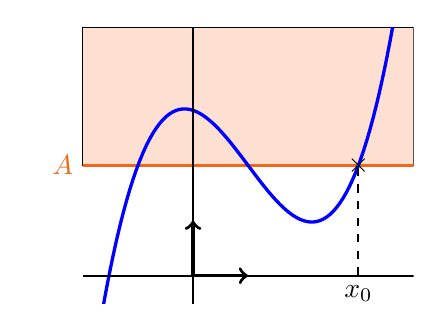
\begin{tikzpicture}[scale=0.7]
\clip (-3,-0.5) rectangle (4,4.5);
\draw [fill=ocre!20] (-2,2) -- (4,2) -- (4,4.5) -- (-2,4.5) -- cycle;

\draw [very thick, ocre, domain = -2:37] plot (\x,2);
\draw [blue, very thick,domain=-2:4,samples=100] plot (\x,{\x*\x*\x/3-\x*\x-\x/3+3});

\draw  [ocre](-2,2) node[left] {$A$};
\draw  (3,0) node[below] {$x_0$};
\draw [thick, dashed] (3,0) -- (3,2);
\draw (3,2) node {$\times$};
\draw [thick] (-2,0)--(4,0);
\draw [thick] (0,-2)--(0,5);
\draw [->, very thick] (0,0)--(1,0);
\draw [->,very thick] (0,0)--(0,1);


\end{tikzpicture}
\end{center}
\end{minipage}\end{example}





\begin{definition}On suppose qu'il existe un réel $a$ tel que $]-\infty ; a ] \subset D$.
\begin{itemize}
\item On dit que $f$ a pour limite $+\infty$ en $-\infty$ si, pour tout réel $A$, il existe un réel $x_0 \in D$ tel que, pour tout $x \in D$, si $x  \leqslant x_0$, alors $f(x) \geqslant A$. On notera $\displaystyle \lim_{x \to -\infty} f(x)=+\infty$.
\item On dit que $f$ a pour limite $-\infty$ en $-\infty$ si, pour tout réel $A$, il existe un réel $x_0 \in D$ tel que, pour tout $x \in D$, si $x  \leqslant x_0$, alors $f(x) \leqslant A$. On notera $\displaystyle \lim_{x \to -\infty} f(x)=-\infty$.\end{itemize}\end{definition}

\begin{example}
 On représente ici une fonction $f$ dans un repère.
 
\begin{minipage}{0.55\linewidth}
 Pour n'importe quel $A$, aussi grand que l'on veut, on peut trouver un $x_0$ en-dessous duquel la courbe est toujours au-dessus de la droite d'équation $y=A$. 

On a  $\displaystyle \lim_{x \to -\infty} f(x)=+\infty$ .

\end{minipage}\hfill\begin{minipage}{0.35\linewidth}
\begin{center}
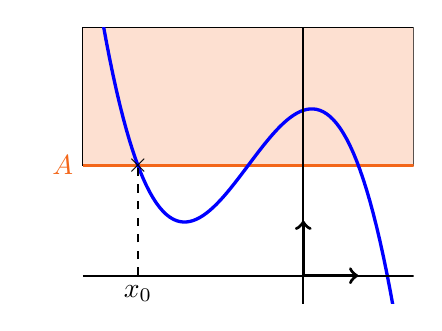
\begin{tikzpicture}[scale=0.7]
\clip (-5,-0.5) rectangle (2,4.5);
\draw [fill=ocre!20] (-4,2) -- (2,2) -- (2,4.5) -- (-4,4.5) -- cycle;

\draw [very thick, ocre, domain = -4:37] plot (\x,2);
\draw [blue, very thick,domain=-4:2,samples=100] plot (\x,{-\x*\x*\x/3-\x*\x+\x/3+3});

\draw  [ocre](-4,2) node[left] {$A$};
\draw  (-3,0) node[below] {$x_0$};
\draw [thick, dashed] (-3,0) -- (-3,2);
\draw (-3,2) node {$\times$};
\draw [thick] (-4,0)--(4,0);
\draw [thick] (0,-2)--(0,5);
\draw [->, very thick] (0,0)--(1,0);
\draw [->,very thick] (0,0)--(0,1);


\end{tikzpicture}
\end{center}
\end{minipage}
\end{example}


Il s'agit de la principale différence avec les suites : pour les suites, l'indice $n$ ne pouvait que tendre vers $+\infty$. Dans le cas des fonctions, le réel $x$ peut aller vers $+\infty$ mais aussi $-\infty$ et d'autres valeurs réelles entre les deux, comme nous le verrons plus tard dans ce chapitre...


\subsection{Limite finie en l'infini}

\begin{definition}On suppose qu'il existe un réel $a$ tel que $[a;+\infty [ \subset D$. Soit $l\in\mathbb{R}$.
\begin{itemize}
\item On dit que $f$ a pour limite $\ell$ en $+\infty$ (ou que $f(x)$ tend vers $\ell$ lorsque $x$ tend vers $+\infty$) si, pour tout $\varepsilon>0$, il existe un réel $x_0$ tel que, si $x \geqslant x_0$, alors $f(x) \in ]\ell-\varepsilon ; \ell+\varepsilon [$.\\ Si une telle limite existe, elle est unique. On note alors $\displaystyle \lim_{x \to +\infty} f(x)=\ell$.
\item On dit que $f$ a pour limite $\ell$ en $-\infty$ (ou que $f(x)$ tend vers $\ell$ lorsque $x$ tend vers $-\infty$) si, pour tout $\varepsilon>0$, il existe un réel $x_0$ tel que, si $x \leqslant x_0$, alors $f(x) \in ]\ell-\varepsilon ; \ell+\varepsilon [$.\\ Si une telle limite existe, elle est unique. On note alors $\displaystyle \lim_{x \to -\infty} f(x)=\ell$.
\end{itemize}\end{definition}

\begin{example} Une fonction $f$ est représentée ci-dessous. Pour n'importe quel $\varepsilon>0$, on peut trouver un réel $x_0$ à partir duquel on a toujours $f(x) \in ]2-\varepsilon ; 2+\varepsilon [$. On a  $\displaystyle \lim_{x \to +\infty} f(x)=2$.

\begin{center}

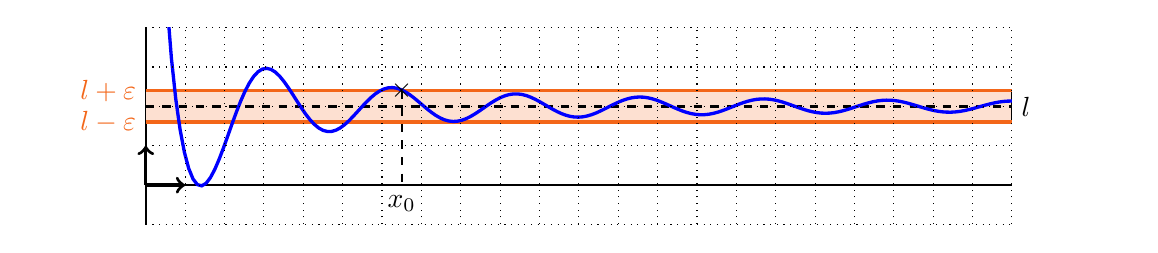
\begin{tikzpicture}[scale=0.5]
\clip (-3,-1) rectangle (25,4);
\draw [thick] (0,0)--(22,0);
\draw [thick] (0,-2)--(0,28);
\draw [->, very thick] (0,0)--(1,0);
\draw [->,very thick] (0,0)--(0,1);

\draw [fill=ocre!20] (0,1.6) -- (22,1.6) -- (22,2.4) -- (0,2.4) -- cycle;
\draw [very thick, ocre, domain = 0:22] plot (\x,1.6);
\draw [very thick, ocre, domain = 0:22] plot (\x,2.4);
\draw [very thick, dashed, domain = 0:22] plot (\x,2);
\draw [very thick, blue, domain = 0.1:22, samples =200] plot (\x,{2+3*cos(2*deg(\x))/\x}) ;
\draw [ thin, dotted] (0,-2) grid (22,28);
\draw  [thick] (6.5,2.4) node {$\times$};
\draw [thick, dashed] (6.5, 2.4) -- (6.5,0);
\draw  [thick] (6.5,0) node[below] {$x_0$};

\draw  [ocre](0,1.6) node[left] {$l-\varepsilon$};
\draw  [ocre](0,2.4) node[ left] {$l+\varepsilon$};
\draw  (22,2) node[right] {$l$};

\end{tikzpicture}
\end{center}\end{example}


\begin{definition} On se place dans un repère $(0;\vec i, \vec j)$ orthonormé.
\begin{itemize}
\item Si $\displaystyle \lim_{x \to +\infty} f(x)=\ell$, on dit que la droite d'équation $y=l$ est asymptote à la courbe de $f$ en $+\infty$
\item Si $\displaystyle \lim_{x \to -\infty} f(x)=\ell$, on dit que la droite d'équation $y=l$ est asymptote à la courbe de $f$ en $-\infty$\end{itemize} \end{definition}

\begin{example}Dans le cas précédent, la droite d'équation $y=2$ est asymptote à la courbe de $f$ en $+\infty$.\end{example}


Comme dans le cas des suites, il est parfois utile de préciser le comportement d'une fonction qui admet une limite finie en $+\infty$.

\begin{definition}On suppose qu'il existe un réel $a$ tel que $[a;+\infty [ \subset D$. Soit $l\in\mathbb{R}$.
\begin{itemize}
\item On dit que $f(x)$ tend vers $\ell$ par valeurs supérieures lorsque $x$ tend vers $+\infty$ si, pour tout $\varepsilon>0$, il existe un réel $x_0$ tel que, si $x \geqslant x_0$, alors $f(x) \in ]\ell ; \ell+\varepsilon [$. Autrement dit, la limite de $f$ en $+\infty$ vaut $\ell$ et $f(x)$ reste supérieur à $\ell$ à partir d'un certain réel. On note alors $\displaystyle \lim_{x \to +\infty} f(x)=\ell^+$.
\item On dit que $f(x)$ tend vers $\ell$ par valeurs inférieures lorsque $x$ tend vers $+\infty$ si, pour tout $\varepsilon>0$, il existe un réel $x_0$ tel que, si $x \geqslant x_0$, alors $f(x) \in ]\ell-\varepsilon ; \ell [$. Autrement dit, la limite de $f$ en $+\infty$ vaut $\ell$ et $f(x)$ reste inférieur à $\ell$ à partir d'un certain réel. On note alors $\displaystyle \lim_{x \to +\infty} f(x)=\ell^-$.
\end{itemize}\end{definition}

Attention, ce n'est pas parce que $\displaystyle \lim_{x \to +\infty} f(x)=\ell$ qu'on a forcément $\displaystyle \lim_{x \to +\infty} f(x)=\ell^+$ ou $\displaystyle \lim_{x \to +\infty} f(x)=\ell^-$. Les valeurs de $f(x)$ peuvent osciller autour de $\ell$, lui étant parfois supérieures, parfois inférieures.

Les mêmes définitions s'étendent naturellement pour les limites en $-\infty$.

\begin{example}On a représenté la courbe d'une fonction $f$ dans un repère.

\begin{minipage}{0.65\linewidth}
Il semblerait que $\displaystyle\lim_{x\to +\infty}f(x)=\qquad$ et $\displaystyle\lim_{x\to -\infty}f(x)=\qquad$

La droite d'équation $y=2$ est asymptote à la courbe de $f$ en $+\infty$.

La droite d'équation $y=-1$ est asymptote à la courbe de $f$ en $-\infty$.
\end{minipage}\hfill \begin{minipage}{0.3\linewidth}
\begin{flushright}

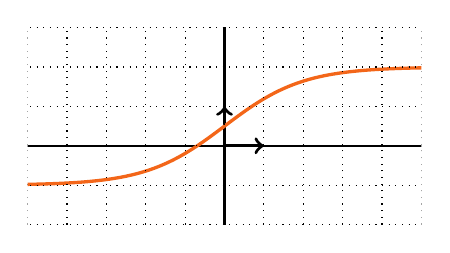
\begin{tikzpicture}[scale=0.5]
\clip (-5,-2) rectangle (5,3);
\draw [thick] (-10,0)--(22,0);
\draw [thick] (0,-2)--(0,28);
\draw [->, very thick] (0,0)--(1,0);
\draw [->,very thick] (0,0)--(0,1);

\draw [very thick, ocre, domain = -5:5, samples =200] plot (\x,{3/(1+exp(-\x))-1}) ;
\draw [thin, dotted] (-10,-2) grid (22,28);

\end{tikzpicture}
\end{flushright}\end{minipage}\end{example}


\subsection{Limites usuelles}

\begin{proposition}Soit $n$ un entier naturel non nul.
\[\displaystyle \lim_{x \to +\infty} x^n = \qquad \qquad \displaystyle \lim_{x \to +\infty} \dfrac{1}{x^n} = \]
\textbf{Si $n$ est pair}, \[\displaystyle \lim_{x \to -\infty} x^n =  \qquad \qquad \displaystyle \lim_{x \to -\infty} \dfrac{1}{x^n}=\]
\textbf{Si $n$ est impair}, 
\[\displaystyle \lim_{x \to -\infty} x^n =  \qquad \qquad \displaystyle \lim_{x \to -\infty} \dfrac{1}{x^n}=\]
Enfin, 
\[\displaystyle \lim_{x \to +\infty} \sqrt{x} =  \qquad \qquad \displaystyle \lim_{x \to +\infty} \e^x =  \qquad \qquad \displaystyle \lim_{x \to -\infty} \e^x = \]
\end{proposition}

Il est important de visualiser les courbes représentatives de ces fonctions. Celles-ci vous permettront de bien garder ces limites usuelles en tête.

\begin{minipage}{0.2\linewidth}
\begin{center}
\textbf{$x \mapsto x^n$, $n$ pair}
\end{center}
\begin{center}
\begin{tikzpicture}[scale=0.45]
\clip (-4,-1) rectangle (4,4);
\draw [thick] (-4,0)--(7,0);
\draw [thick] (0,-4) -- (0,5);
\draw [very thick,->,>=latex] (0,0)--(0,1);
\draw [very thick,->,>=latex] (0,0)--(1,0);
\end{tikzpicture}
\end{center}
\end{minipage}\hfill\begin{minipage}{0.2\linewidth}

\begin{center}
\textbf{$x \mapsto \frac{1}{x^n}$, $n$ pair}
\end{center}
\begin{center}
\begin{tikzpicture}[scale=0.45]
\clip (-4,-1) rectangle (4,4);
\draw [thick] (-4,0)--(7,0);
\draw [thick] (0,-4) -- (0,5);
\draw [very thick,->,>=latex] (0,0)--(0,1);
\draw [very thick,->,>=latex] (0,0)--(1,0);
\end{tikzpicture}
\end{center}
\end{minipage}\hfill
\begin{minipage}{0.2\linewidth}
\begin{center}
\textbf{$x \mapsto \e^x$}
\end{center}
\begin{center}
\begin{tikzpicture}[scale=0.45]
\clip (-4,-1) rectangle (4,4);
\draw [thick] (-4,0)--(7,0);
\draw [thick] (0,-4) -- (0,5);
\draw [very thick,->,>=latex] (0,0)--(0,1);
\draw [very thick,->,>=latex] (0,0)--(1,0);
\end{tikzpicture}
\end{center}\end{minipage}


\vskip10pt

\begin{minipage}{0.2\linewidth}
\begin{center}
\textbf{$x \mapsto x^n$, $n$ impair}
\end{center}
\begin{center}
\begin{tikzpicture}[scale=0.45]
\clip (-4,-3) rectangle (4,3);
\draw [thick] (-4,0)--(7,0);
\draw [thick] (0,-4) -- (0,5);
\draw [very thick,->,>=latex] (0,0)--(0,1);
\draw [very thick,->,>=latex] (0,0)--(1,0);
\end{tikzpicture}
\end{center}
\end{minipage}\hfill\begin{minipage}{0.2\linewidth}
\begin{center}
\textbf{$x \mapsto \frac{1}{x^n}$, $n$ impair}
\end{center}
\begin{center}
\begin{tikzpicture}[scale=0.45]
\clip (-4,-3) rectangle (4,3);
\draw [thick] (-4,0)--(7,0);
\draw [thick] (0,-4) -- (0,5);
\draw [very thick,->,>=latex] (0,0)--(0,1);
\draw [very thick,->,>=latex] (0,0)--(1,0);
\end{tikzpicture}
\end{center}
\end{minipage}\hfill\begin{minipage}{0.2\linewidth}
\begin{center}
\textbf{$x \mapsto \sqrt{x}$}
\end{center}
\begin{center}
\begin{tikzpicture}[scale=0.45]
\clip (-4,-3) rectangle (4,3);
\draw [thick] (-4,0)--(7,0);
\draw [thick] (0,-4) -- (0,5);
\draw [very thick,->,>=latex] (0,0)--(0,1);
\draw [very thick,->,>=latex] (0,0)--(1,0);
\end{tikzpicture}
\end{center}
\end{minipage}




\section{Limite en un point}

\subsection{Limite finie en un point}

\begin{definition}Soit $a \in D$ et $l$ un réel.

On dit que $f(x)$ tend vers $\ell$ lorsque $x$ tend vers $a$  si, pour tout $\varepsilon>0$, il existe un réel $\delta >0$ tel que, si $x\in ]a - \delta ; a+\delta[$, alors $f(x) \in ]\ell-\varepsilon : \ell+ \varepsilon [$.

Autrement dit, tout intervalle ouvert centré en $\ell$ contient toutes les valeurs de $x$ lorsque $x$ est suffisamment proche de $a$.

Si elle existe, une telle limite est unique. On note alors $\displaystyle \lim_{x \to a} f(x) =\ell $\end{definition}

Certaines fonctions admettent une limite finie différente si l'on se rapproche de $a$ par valeurs supérieurs ou par valeurs inférieures. Nous aurons l'occasion d'en discuter plus amplement dans le chapitre suivant.

\subsection{Limite infinie en un point}

\begin{definition}Soit $a \in D$ ou sur un bord de $D$.
\begin{itemize}
\item On dit que $f(x)$ tend vers $+\infty$ lorsque $x$ tend vers $a$  si, pour tout réel $A$, il existe un réel $\delta >0$ tel que, si $x\in ]a - \delta ; a+\delta[\cap D$, alors $f(x) > A$. Autrement dit, l'intervalle $]A;+\infty[$ contient toutes les valeurs de $f(x)$ lorsque $x$ est suffisamment proche de $a$. On note alors $\displaystyle \lim_{x \to a} f(x) =+\infty $.
\item On dit que $f(x)$ tend vers $-\infty$ lorsque $x$ tend vers $a$  si, pour tout réel $A$, il existe un réel $\delta >0$ tel que, si $x\in ]a - \delta ; a+\delta[\cap D$, alors $f(x) < A$. On note alors $\displaystyle \lim_{x \to a} f(x) =-\infty $.
\end{itemize}
\end{definition}

\begin{example} On a tracé ci-dessous la représentation graphique d'une fonction $f$.

\begin{center}

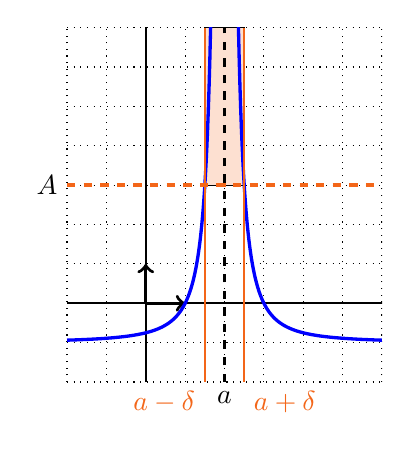
\begin{tikzpicture}[scale=0.5]
\clip (-3,-3) rectangle (6,7);
\draw [thick] (-2,0)--(22,0);
\draw [thick] (0,-2)--(0,28);
\draw [->, very thick] (0,0)--(1,0);
\draw [->,very thick] (0,0)--(0,1);
\draw [ thin, dotted] (-2,-2) grid (22,28);

\draw [fill=ocre!20] (1.5,3) -- (2.5,3) -- (2.5,7) -- (1.5,7) -- cycle;
\draw [very thick, blue, domain = -2:1.8, samples =200] plot (\x,{1/((\x-2)*(\x-2))-1}) ;
\draw [very thick, blue, domain = 2.2:6, samples =200] plot (\x,{1/((\x-2)*(\x-2))-1}) ;

\draw [very thick,ocre, dashed, domain = -2:22] plot (\x,3);

\draw [thick, ocre] (1.5,-2) -- (1.5,7);
\draw [thick, ocre] (2.5,-2) -- (2.5,7);
\draw [very thick, dashed] (2,-2) -- (2,7);

\draw  [ocre](1.5,-2) node[below left] {$a-\delta$};
\draw  [ocre](2.5,-2) node[below right] {$a+\delta$};
\draw  (2,-2) node[below] {$a$};
\draw  (-2,3) node[left] {$A$};

\end{tikzpicture}
\end{center}

Pour n'importe quelle valeur du réel $A$, on peut trouver un intervalle centré sur $a$ tel que toute valeur de $f(x)$ est supérieur à $A$ pour n'importe quel $x$ pris dans cet intervalle. Ce raisonnement vaut peu importe la valeur du réel $A$ : on a $\displaystyle \lim_{x \to a} f(x) =+\infty $.\end{example}


Tout comme précédemment, le comportement de la fonction $f$ peut varier selon si l'on approche du réel $a$ par valeurs inférieures ou supérieures. Il nous faut donc distinguer ces deux cas.

\newpage

\begin{definition}Soit $a \in D$ ou sur un bord de $D$.
\begin{itemize}
\item On dit que $f(x)$ tend vers $+\infty$ lorsque $x$ tend vers $a$ par valeurs inférieures  si, pour tout réel $A$, il existe un réel $\delta >0$ tel que, si $x\in ]a - \delta ; a[\cap D$, alors $f(x) > A$. Autrement dit, l'intervalle $]A;+\infty[$ contient toutes les valeurs de $f(x)$ lorsque $x$ est suffisamment proche de $a$ tout en lui étant inférieur. On note alors $\displaystyle \lim_{x \to a^-} f(x) =+\infty $.
\item On dit que $f(x)$ tend vers $+\infty$ lorsque $x$ tend vers $a$ par valeurs supérieures  si, pour tout réel $A$, il existe un réel $\delta >0$ tel que, si $x\in ]a ; a+\delta[\cap D$, alors $f(x) > A$. Autrement dit, l'intervalle $]A;+\infty[$ contient toutes les valeurs de $f(x)$ lorsque $x$ est suffisamment proche de $a$ tout en lui étant supérieur. On note alors $\displaystyle \lim_{x \to a^+} f(x) =+\infty $.
\end{itemize}
\end{definition}

Là encore, ces définitions peuvent s'étendre pour une limite valant $-\infty$.


\begin{example} On considère la fonction $f:x\mapsto \dfrac{1}{x-1}$, définie sur $\mathbb{R} \setminus \{1\}$, dont on a tracé ci-dessous la courbe dans un repère.

\begin{minipage}{0.3\linewidth}
\begin{center}

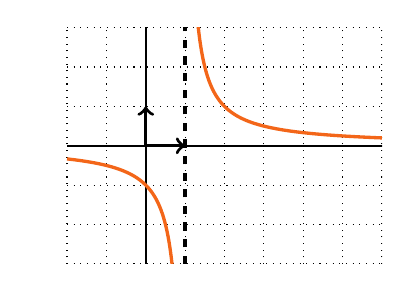
\begin{tikzpicture}[scale=0.5]
\clip (-3,-3) rectangle (6,3);
\draw [thick] (-2,0)--(22,0);
\draw [thick] (0,-3)--(0,28);
\draw [->, very thick] (0,0)--(1,0);
\draw [->,very thick] (0,0)--(0,1);
\draw [ thin, dotted] (-2,-3) grid (22,28);

\draw [very thick, ocre, domain = -2:0.8, samples =200] plot (\x,{1/(\x-1)}) ;
\draw [very thick, ocre, domain = 1.2:6, samples =200] plot (\x,{1/((\x-1)}) ;

\draw [very thick, dashed] (1,-3) -- (1,7);


\end{tikzpicture}
\end{center}
\end{minipage}\hfill\begin{minipage}{0.65\linewidth}

Il semblerait que, lorsque l'on s'approche de $1$ par valeurs supérieures, la limite soit $+\infty$, ce que l'on notera $\displaystyle \lim_{x \to 1^+} f(x) =+\infty $.
\vskip5pt
En revanche, lorsque l'on s'approche de $1$ par valeurs inférieures, la limite semble être $-\infty$, ce que l'on note $\displaystyle \lim_{x \to 1^-} f(x) =-\infty $. \end{minipage}
\end{example}



\begin{definition}Lorsque la limite d'une fonction $f$ est infinie en un point $a$, on dit que la droite d'équation $x=a$ est une asymptote verticale à la courbe représentative de $f$.\end{definition}

\begin{example} Dans l'exemple précédent, la droite d'équation $x=1$ est asymptote à la courbe de $f$.\end{example}


\section{Opérations sur les limites}

Les opérations sur les limites sont similaires à celles connues sur les suites. Dans cette partie, $f$ et $g$ sont deux fonctions définies au voisinages de $a$, $a$ pouvant être un réel, $+\infty$ ou $-\infty$. $l_1$ et $l_2$ sont deux réels.

\subsection{Limite de la somme}

\begin{proposition}[Limite de la somme] On a :

\begin{center}
\begin{tabularx}{\linewidth}{|l|X|X|X|X|X|X|}
\hline
$\displaystyle \lim_{x \to a} f(x)$ & $l_1$ & $l_1$ & $l_1$ & $+\infty$ & $-\infty$ & $ +\infty$\\
\hline
$\displaystyle \lim_{x \to a} g(x)$ & $l_2$ & $+\infty$ & $-\infty$ & $+\infty$ & $-\infty$ & $-\infty$ \\
\hline
$\displaystyle \lim_{x \to a} (f(x)+g(x))$ &  &  &  &  &   & \textbf{FI}\\
\hline
\end{tabularx}
\end{center}\end{proposition}

\newpage


\subsection{Limite du produit}


\begin{proposition}[Limite du produit].
\begin{center}

\begin{tabularx}{\linewidth}{|l|X|X|X|X|}
\hline
$\displaystyle \lim_{x \to a} f(x)$ & $l_1 $ & $l_1 \neq 0$ & $\infty$ & $0$ \\
\hline
$\displaystyle \lim_{x \to a} g(x)$ & $l_2$ & $\infty$ &  $\infty$ & $\infty$ \\
\hline
$\displaystyle \lim_{x \to a} (f(x)\,g(x))$ &  &  &  &  \\
\hline
\end{tabularx}

 \textbf{r.s. : Règle des signes}
 \end{center} \vspace{-1cm}
\end{proposition}

\begin{example}On considère la fonction $f$ définie pour tout réel $x$ non nul par $f(x)=x^2-x+\dfrac{1}{x}$.
\vskip120pt

\end{example}

\subsection{Limite du quotient}

\begin{proposition}[Limite du quotient] Dans cette partie, on suppose $l_2 \neq 0$.
\begin{center}

\begin{tabularx}{\linewidth}{|l|X|X|X|X|X|X|}
\hline
$\displaystyle \lim_{x \to a} f(x)$ & $l_1 $ & $l_1$ & $l_1 \neq 0$ & $\infty$ & 0 & $\infty$ \\
\hline
$\displaystyle \lim_{x \to a} g(x)$ & $l_2$ & $\infty$ &  $0^+$ ou $0^-$ & $l_2$, $0^+$ ou $0^-$  & $0$ & $\infty$ \\
\hline
$\displaystyle \lim_{x \to a} \left(\dfrac{f(x)}{g(x)}\right)$ &  &  &  &  & &  \\
\hline
\end{tabularx}

 \textbf{r.s. : Règle des signes}
 \end{center} \vspace{-1cm}
\end{proposition}

\begin{example}Pour tout réel $x$, on pose $f(x)=\dfrac{1-2x^4}{1+x^2}$. L'étude des limites en $+\infty$ et $-\infty$ de $f$ aboutit à une forme indéterminée. Or, pour tout réel non nul $x$,
\[f(x)= \]

\vskip80pt
\end{example}
\newpage
\begin{example}On considère la fonction $f$ définie pour tout réel $x\neq 2$ par $f(x)=\dfrac{3x+1}{2x-4}$.

\vskip100pt

\end{example}


\begin{example} On considère la fonction $f:x\mapsto \sqrt{x} + \dfrac{1}{1-x}$, définie sur $[0;1[ \cup ]1;+\infty[$.

\textbf{Pour calculer la limite en $1^+$ :}
\begin{itemize}
\item $\displaystyle \lim_{x \to 1^+} \sqrt{x} = $.
\item $\displaystyle \lim_{x \to 1} (1-x)=\qquad$. Par ailleurs, si $x \geqslant 1$, alors $1-x \leqslant 0$ et donc $\displaystyle \lim_{x \to 1^+} (1-x)=\qquad $. 

Ainsi, par quotient de limites, $\displaystyle \lim_{x \to 1^+} \dfrac{1}{1-x}=\qquad$.
\item Par somme de limites, $\displaystyle \lim_{x \to 1^+} f(x)=\qquad$.

\end{itemize}


\textbf{Pour calculer la limite en $1^-$ :}
\begin{itemize}
\item $\displaystyle \lim_{x \to 1^-} \sqrt{x} = \qquad $.
\item $\displaystyle \lim_{x \to 1} (x-1)=\qquad $. Par ailleurs, si $x \leqslant 1$, alors $1-x \geqslant 0$ et donc $\displaystyle \lim_{x \to 1^-} (1-x)=\qquad $. 

Ainsi, par quotient de limites, $\displaystyle \lim_{x \to 1^+} \dfrac{1}{1-x}=\qquad$.
\item Par somme de limites, $\displaystyle \lim_{x \to 1^-} f(x)=\qquad$.
\end{itemize}

\textbf{Pour calculer la limite en $+\infty$ :}
\begin{itemize}
\item $\displaystyle \lim_{x \to +\infty} \sqrt{x} =\qquad$. 
\item $\displaystyle \lim_{x \to +\infty} (1-x)= \qquad$, ainsi, par quotient de limites, $\displaystyle \lim_{x \to +\infty} \dfrac{1}{1-x}=\qquad$.
\item Par somme de limites, $\displaystyle \lim_{x \to +\infty} f(x)=\qquad$.
\end{itemize}

Représenter la courbe de la fonction $f$ dans un graphique (par exemple, dans un logiciel de géométrie ou sur une calculatrice) permet de confirmer ou d'infirmer les calculs.


\begin{center}
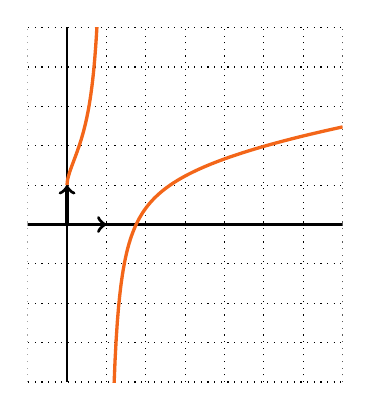
\begin{tikzpicture}[scale=0.5]
\clip (-1,-4) rectangle (7,5);
\draw [thick] (-2,0)--(22,0);
\draw [thick] (0,-4)--(0,28);
\draw [->, very thick] (0,0)--(1,0);
\draw [->,very thick] (0,0)--(0,1);
\draw [ thin, dotted] (-2,-4) grid (22,28);

\draw [very thick, ocre, domain = 0:0.9, samples =200] plot (\x,{sqrt(\x)+1/(1-\x)}) ;
\draw [very thick, ocre, domain = 1.1:7, samples =200] plot (\x,{{sqrt(\x)+1/(1-\x)}}) ;


\end{tikzpicture}
\end{center}
\vspace{-1cm}
\end{example}
\newpage 
\subsection{Composition de limites}

\begin{proposition}Soit $a$, $b$ et $c$ des réels ou $\pm \infty$. Soit $f$ et $g$ des fonctions définies sur $\mathbb{R}$.
On suppose que $\displaystyle\lim_{x \to a}f(x)=b$ et $\displaystyle\lim_{X \to b}g(X)=c$. Alors $\displaystyle\lim_{x \to a}(g \circ f)(x)=c$.
\end{proposition}


\begin{example} On considère la fonction $f:x\mapsto \e^{-2x^2-3x-5}$. 
\vskip50pt
\end{example}



\section{Comparaison de limites}

\begin{theorem}[Théorème de comparaison]Soit $a$ un réel ou $\pm \infty$. Soit $f$ et $g$ deux fonctions définies sur un intervalle $I$ dont $a$ est un élément ou un bord.
\begin{itemize}
\item Si, pour tout $x\in I$, $f(x)\geqslant g(x)$ et $\displaystyle \lim_{x \to a} g(x)=+\infty$, alors $\displaystyle \lim_{x \to a} f(x)=+\infty$.
\item Si, pour tout $x\in I$, $f(x)\leqslant g(x)$ et $\displaystyle \lim_{x \to a} g(x)=-\infty$, alors $\displaystyle \lim_{x \to a} f(x)=-\infty$.
\end{itemize}\end{theorem}

\begin{example}Pour tout réel $x$, on pose $f(x)=(2+\cos(x))\e^x$. 

\vskip80pt
\end{example}

\begin{example}On souhaite montrer que, justement, $\displaystyle \lim_{x \to +\infty}\e^x=+\infty$. 

\vskip180pt
\end{example}

\newpage


\begin{theorem}[Théorème d'encadrement]Soit $a$ un réel. Soit $f$, $g$ et $h$ trois fonctions définies sur un intervalle $I$ dont $a$ est un élément ou un bord.

Si, pour tout $x\in I$, $f(x)\leqslant g(x)\leqslant$ et si $f$ et $h$ admettent une même limite \textbf{finie} $l$ en $a$, alors $g$ admet également une limite finie en $a$ et $\displaystyle \lim_{x \to +\infty} g(x)=l$.
\end{theorem}

\begin{example}Pour tout réel non nul $x$, on pose $f(x)=\dfrac{\cos(x)}{x}$.

 \vskip50pt
 \end{example}
 
\begin{example}Pour tout réel non nul $x$, on pose $g(x)=x\,\sin\left(\dfrac{1}{x}\right)$. On souhaite déterminer $\displaystyle\lim_{x \to 0^+}f(x)$.

\vskip50pt
\end{example}


\section{Croissances comparées}

\begin{proposition}[Croissances comparées -- fonction exponentielle] Soit $n$ un entier naturel.
\[\displaystyle \lim_{x \to +\infty} \dfrac{\e^x}{x^n}=+\infty \qquad \qquad \displaystyle \lim_{x \to -\infty} x^n\,\e^x =0\]

\vspace{-0.5cm}\end{proposition}


\begin{example} Pour tout réel $x$, on pose $f(x)=\dfrac{\e^x-x}{\e^x}$.
\vskip40pt
\end{example}

Cette proposition peut être vue comme la limite de nouvelles fonctions, les fonctions $x\mapsto \dfrac{\e^x}{x^n}$ et $x\mapsto x^n\,\e^x$. Il est alors possible d'utiliser tous les résultats précédents, en particuliers ceux sur la composition. Par exemple, si l'on considère une fonction $u$ telle que $\displaystyle\lim_{x \to a}u(x)=+\infty$, alors on aura $\displaystyle\lim_{x \to a}\dfrac{\e^{u(x)}}{u(x)}=+\infty$.

\textbf{Il est important de bien avoir la même expression dans l'exponentielle et au dénominateur !}

\begin{example}On considère la fonction $f : x\mapsto \dfrac{\e^{-2x+4}}{3x^3}$, définie sur $\mathbb{R}^*$. On souhaite déterminer $\displaystyle\lim_{x \to -\infty}f(x)$. Pour cela, il semble naturel de faire intervenir une croissance comparée. Seulement, les expressions dans l'exponentielle et au dénominateur sont différentes, il faut donc transformer légèrement cette écriture pour se ramener aux fonctions mentionnées dans la propriété.

Pour tout réel non nul $x$, 
\[\dfrac{\e^{-2x+4}}{3x^3} = \]

\vskip40pt
\end{example}



\section{Approfondissement : Asymptotes obliques}

\begin{definition}Soit $a$ un réel et $f$ une fonction définie sur $]a;+\infty[$. Soit $m$ et $p$ des réels. 

On dit que la droite d'équation $y=mx+p$ est asymptote à la courbe représentative de $f$ en $+\infty$ si \[\displaystyle \lim_{x \to +\infty} (f(x)-(mx+p))=0.\]\end{definition}


\begin{example} On considère la fonction $f:x\mapsto \dfrac{x^2+3x-3}{2x-2}$, définie sur $\mathbb{R}\setminus \{1\}$. Pour tout $x\neq 1$, 
\[f(x)-\left(\dfrac{1}{2}x+2\right)=\dfrac{x^2+3x-3}{2x-2}-\dfrac{\left(\dfrac{1}{2}x+2\right)(2x-2)}{2x-2}=\dfrac{x^2+3x-3-x^2-4x+x+4}{2x-2}=\dfrac{1}{2x-2}.\]

Ainsi, $\displaystyle \lim_{x \to +\infty} \left(f(x)-\left(\dfrac{1}{2}x+2\right)\right)=0$ et $\displaystyle \lim_{x \to -\infty} \left(f(x)-\left(\dfrac{1}{2}x+2\right)\right)=0$. 

La droite d'équation $y=\dfrac{1}{2}x+2$ est asymptote à la courbe représentative de $f$ en $+\infty$ et en $-\infty$.

Il est également possible, en étudiant le signe de $f(x)-\left(\dfrac{1}{2}x+2\right)$, de déterminer la position relative de la courbe de $f$ par rapport à son asymptote.
Ainsi, 
\[ f(x)-\left(\dfrac{1}{2}x+2\right) \leqslant 0 \Leftrightarrow \dfrac{1}{2x-2} \leqslant 0 \Leftrightarrow 2x-2 \leqslant 0 \Leftrightarrow x\leqslant 1.\]

La courbe de $f$ est en-dessous de son asymptote en $-\infty$ et est au-dessus en $+\infty$.

\begin{center}
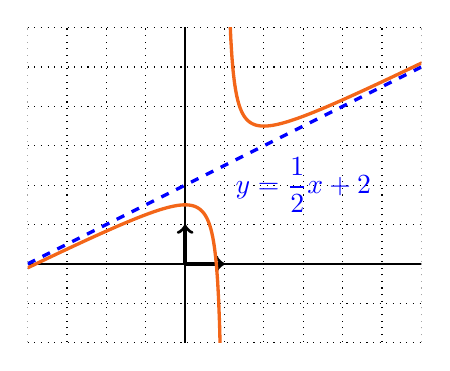
\begin{tikzpicture}[scale=0.5]
\clip (-4,-2) rectangle (6,6);
\draw [thick] (-4,0)--(22,0);
\draw [thick] (0,-4)--(0,28);
\draw [->, very thick] (0,0)--(1,0);
\draw [->,very thick] (0,0)--(0,1);
\draw [ thin, dotted] (-4,-4) grid (22,28);

\draw [very thick, ocre, domain = -4:0.9, samples =200] plot (\x,{(\x*\x+3*\x-3)/(2*\x-2)}) ;
\draw [very thick, ocre, domain = 1.1:7, samples =200] plot (\x,{(\x*\x+3*\x-3)/(2*\x-2)}) ;
\draw [very thick, blue, dashed, domain = -4:7, samples =200] plot (\x,{\x/2+2}) ;
\draw [blue] (3,2) node {$y=\dfrac{1}{2}x+2$};

\end{tikzpicture}
\end{center}
\vspace{-1cm}\end{example}



\end{document}